\section{Derived Triangles}
\label{app:Aderived}

A {\em derived triangle} $T'$ is constructed from the vertices of  a reference triangle $T$. A convenient representation is by a $3\times  3$  matrix, where each row, taken as trilinears, is a vertex of $T'$.




\subsection{Excentral, medial, and intouch triangles}

The {\em  excentral triangle} is the triangle defined by the intersections of the external bisectors of a triangle.

\noindent The {\em medial triangle} is the triangle whose vertices are the midpoints of the vertices of the reference triangle.

\noindent The {\em intouch triangle}  is the triangle whose vertices are the points of tangency of the  incircle centered at $X_1$(incenter) and the sidelines of the reference triangle.



The matrix vertex are given by \cite{mw}: 

%, built from Triangle Center functions $h_1,h_2,h_3$ as follows \cite{kimberling1993_rocky}:

%\begin{align*}
%T'=
%\left[
%\begin{matrix}
%h_1(s_1,s_2,s_3) & h_2(s_1,s_2,s_3) & %h_3(s_1,s_2,s_3)\\ 
%   h_3(s_2,s_3,s_1) & h_1(s_2,s_3,s_1) & %h_2(s_2,s_3,s_1) \\
%   h_2(s_3,s_1,s_2) & h_3(s_3,s_1,s_2) & %h_1(s_3,s_1,s_2)
%\end{matrix}
%\right]
%\end{align*}

\begin{equation*}
\left[
\begin{matrix}
-1&1&1\\1&-1&1\\1&1&-1
\end{matrix}
\right],\;
\left[
\begin{matrix}
0&b^{-1}&c^{-1}\\a^{-1}&0&c^{-1}\\a^{-1}&b^{-1}&0
\end{matrix}
\right],\;
\left[
\begin{matrix}
0&\frac{a c}{a-b+c}&\frac{a b}{a+b-c}\\
\frac{b c}{ b+c-a}&0&\frac{a b}{a+b-c}\\
\frac{b c}{ b+c-a}&\frac{a c}{a-b+c}&0
\end{matrix}
\right]
\end{equation*}

 \subsection{Brocard triangle}
 
 The first Brocard point (resp. second Brocard point)  of a triangle $T=ABC$ (labelled in counterclockwise order) is the unique interior point $\Omega$ such that the angles $\angle\Omega AB$,   $\angle\Omega BC$ and  $\angle\Omega CA$  are equal (resp. the point $\Omega'$ such that the three angles $\angle\Omega' BA$,   $\angle\Omega' CB$ and  $\angle\Omega' AC$ are equal).
 
 The trilinear coordinates of $\Omega$ is $[c/b:a/c:b/a].$ And, the trilinear coordinates of $\Omega'$ is $[b/c:c/a:a/b].$
 
 \begin{figure}[H]
 %   \centering
  % 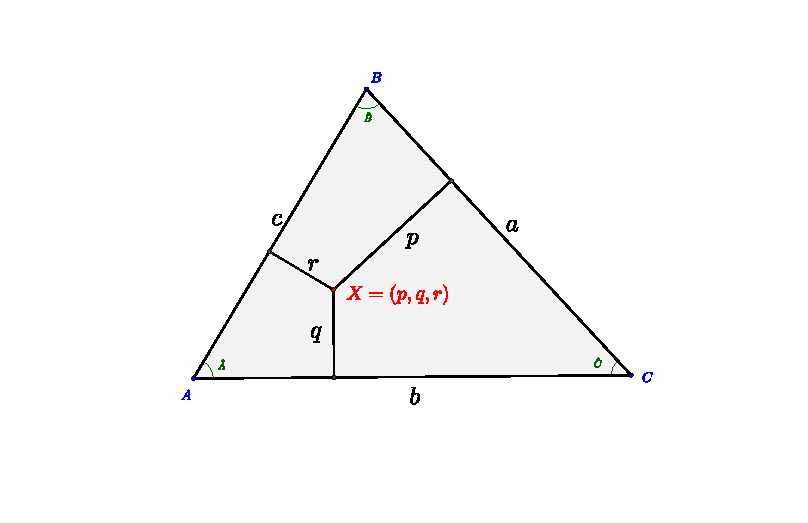
\includegraphics[scale=0.5]{trilinear.pdf}
      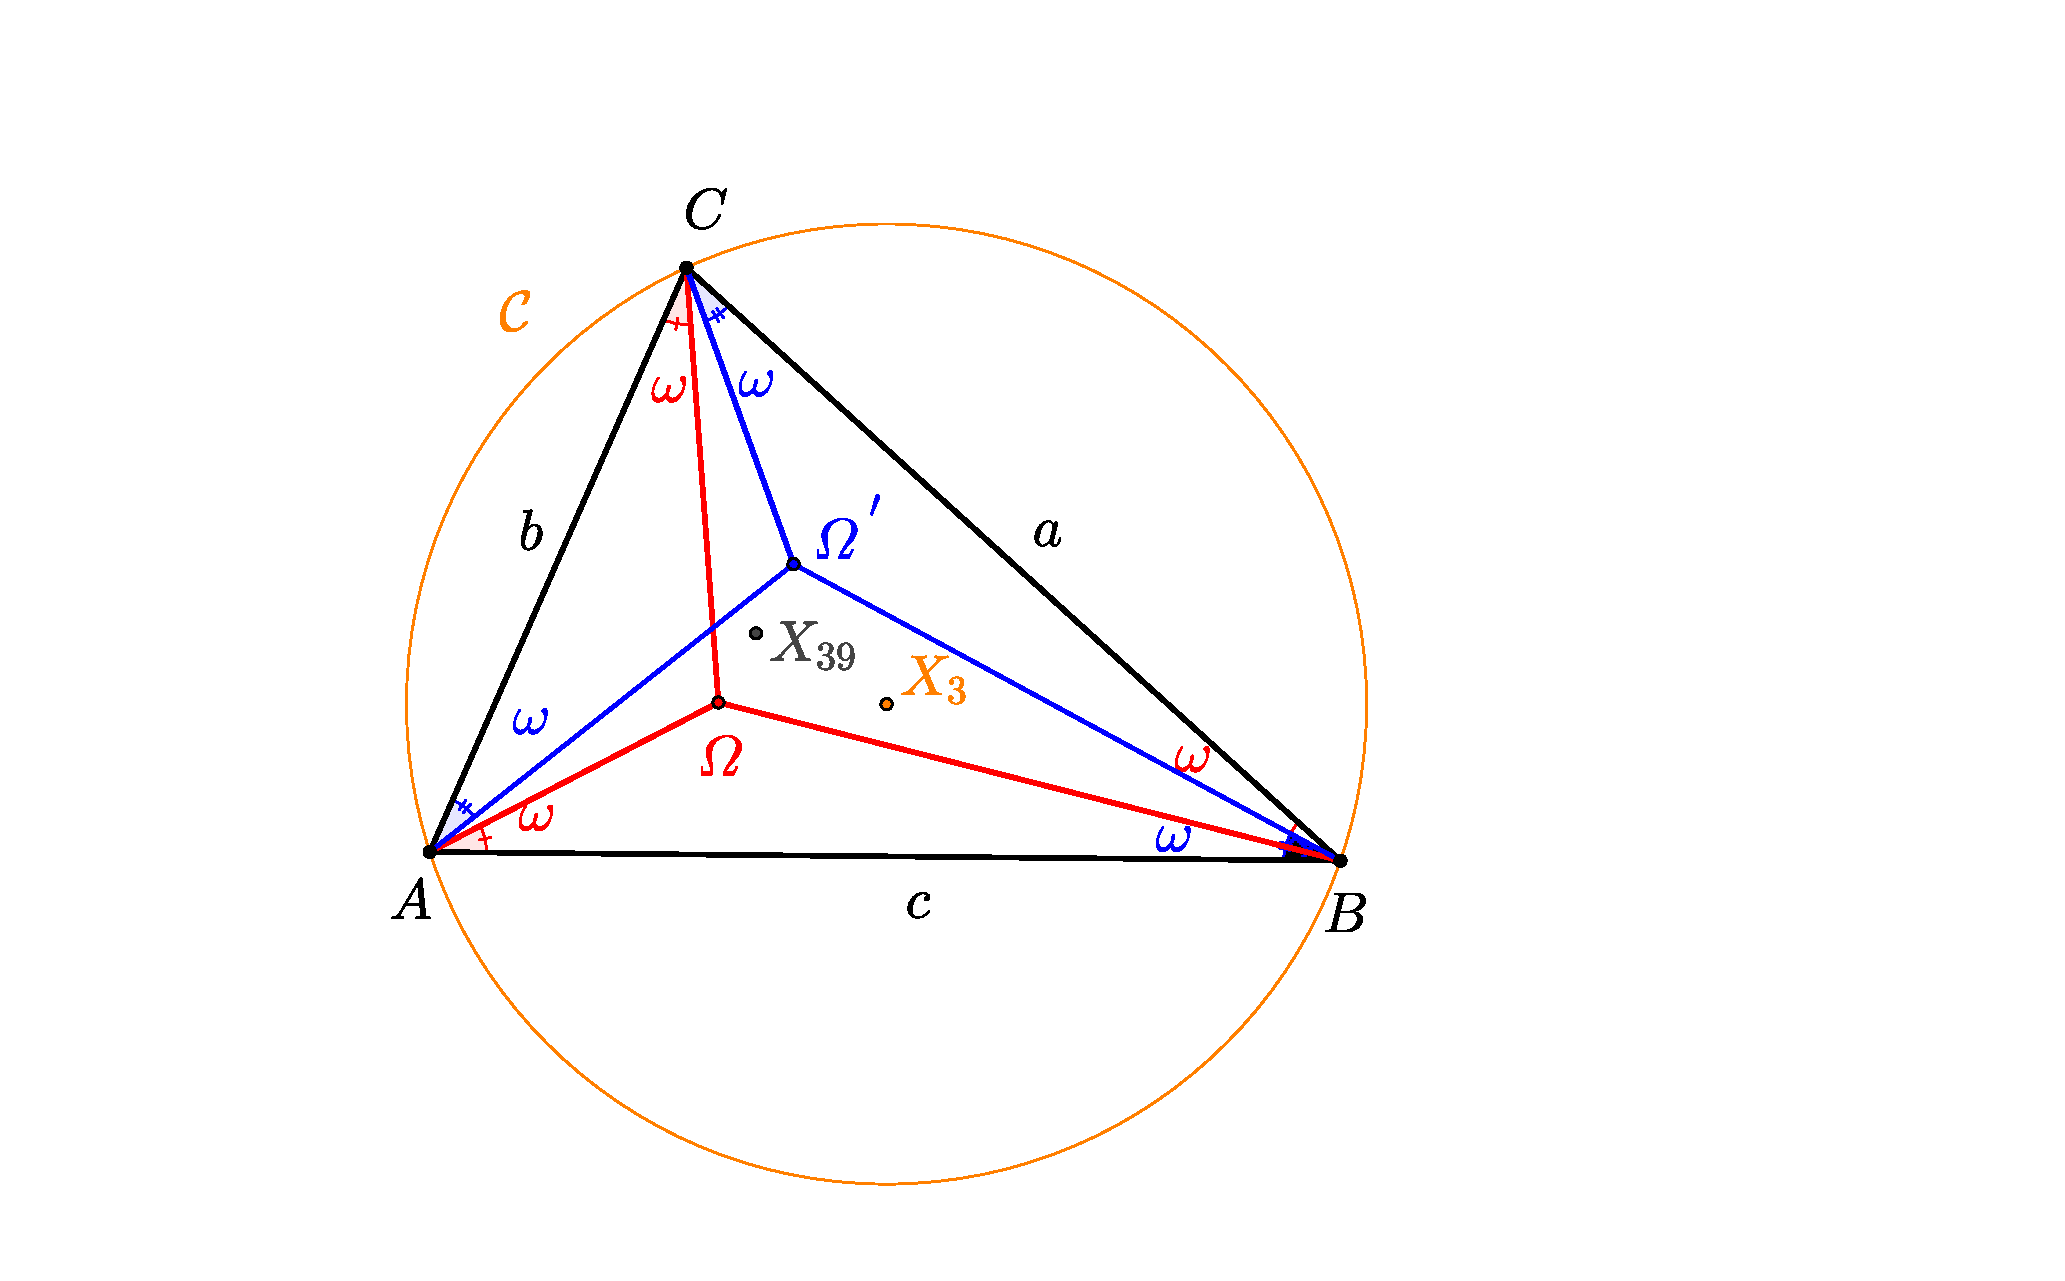
\includegraphics[scale=0.4]{pics_appA_030_brocard_points.pdf}
    \caption{Brocard points $\Omega$ and $\Omega'$ of a triangle $ABC$.}
    \label{fig:brocard_points}
\end{figure}

Consider the six straight lines passing through the vertices $A,B,C$ and the Brocard points $\Omega$ and $\Omega$.

The triangle with vertices $B_1=A\Omega\cap B\Omega'$, $B_2=C\Omega\cap A\Omega'$ and $B_3=B\Omega\cap C\Omega'$ is called the {\em first Brocard triangle}. See \cref{fig:brocard_triangle}.
 \begin{figure}[H]
    \centering
  % 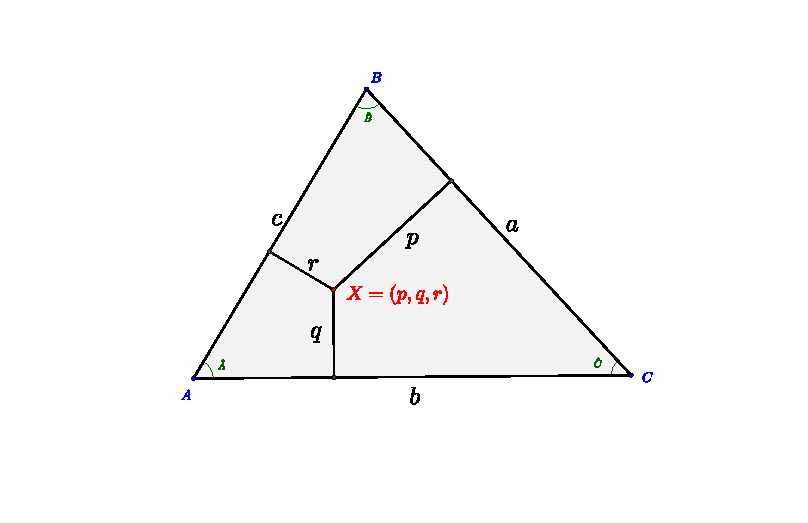
\includegraphics[scale=0.5]{trilinear.pdf}
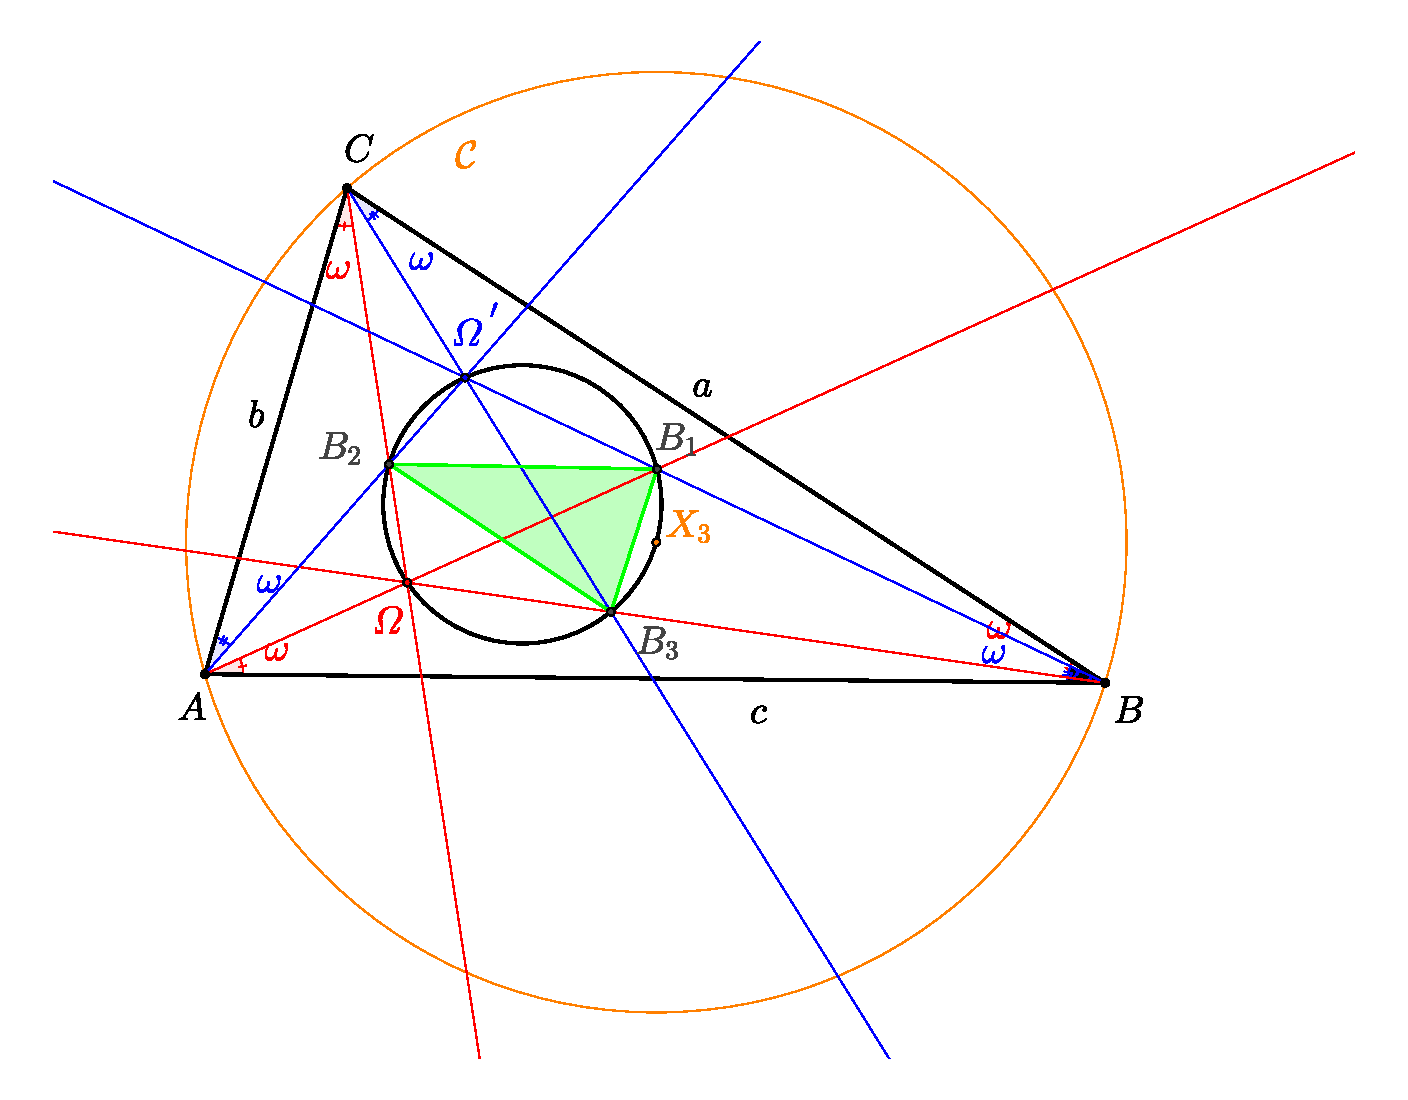
\includegraphics[scale=0.6]{pics_appA_040_brocard_triangle.pdf}
    \caption{Brocard triangle $B_1B_2B_3$ .}
    \label{fig:brocard_triangle}
\end{figure}
The Brocard circle $\mathcal{C}_B$ is the circle passing through the two Brocard points and the $X_3$ (center of the circumcircle of the triangle $ABC$.)
The center of $\mathcal{C}_B$ is  $X_{182}$, which is the middle point of  
the point $X_6$ (symmedian) and $X_{3}.$

The lines $X_3X_6$ and $\Omega\Omega'$ are orthogonal.

Some facts about Brocard points are the following ones. See \cite{johnson29}.

\[ \cot A+\cot B+\cot C=\cot \omega.\]

\[ |\Omega-X_3|=|\Omega'-X_3|=R\sqrt{1-4\sin^2\omega}.\]

\[R_B=\frac{R\sqrt{1-4\sin^2\omega}}{2\cos\omega}.\]

The trilinear vertex matrix of the Brocard triangle $B_1B_2B_3$ is given by:

\begin{align*}
   \left(\begin{matrix} abc& c^3& b^3\\
   c^3&abc & a^3\\
   b^3 &a^3 &abc\end{matrix}\right)
\end{align*}

\subsection{Intouch and extouch triangles}

Given a triangle $T=ABC$ and their incircle,  the intouch triangle (or contact triangle) is the triangle  whose vertices are the contact points of the incircle with the sidelines of $T$. The sidelines of the intouch triangle are the polar lines of the vertices of $T$.

Analogously, the extouch triangle is the triangle whose vertices are   contact points of the sidelines of $T$ with the excircles (circles centered at excenters).

 See \cref{fig:appA-intouch-extouch}.
 \begin{figure}[H]
     \centering
      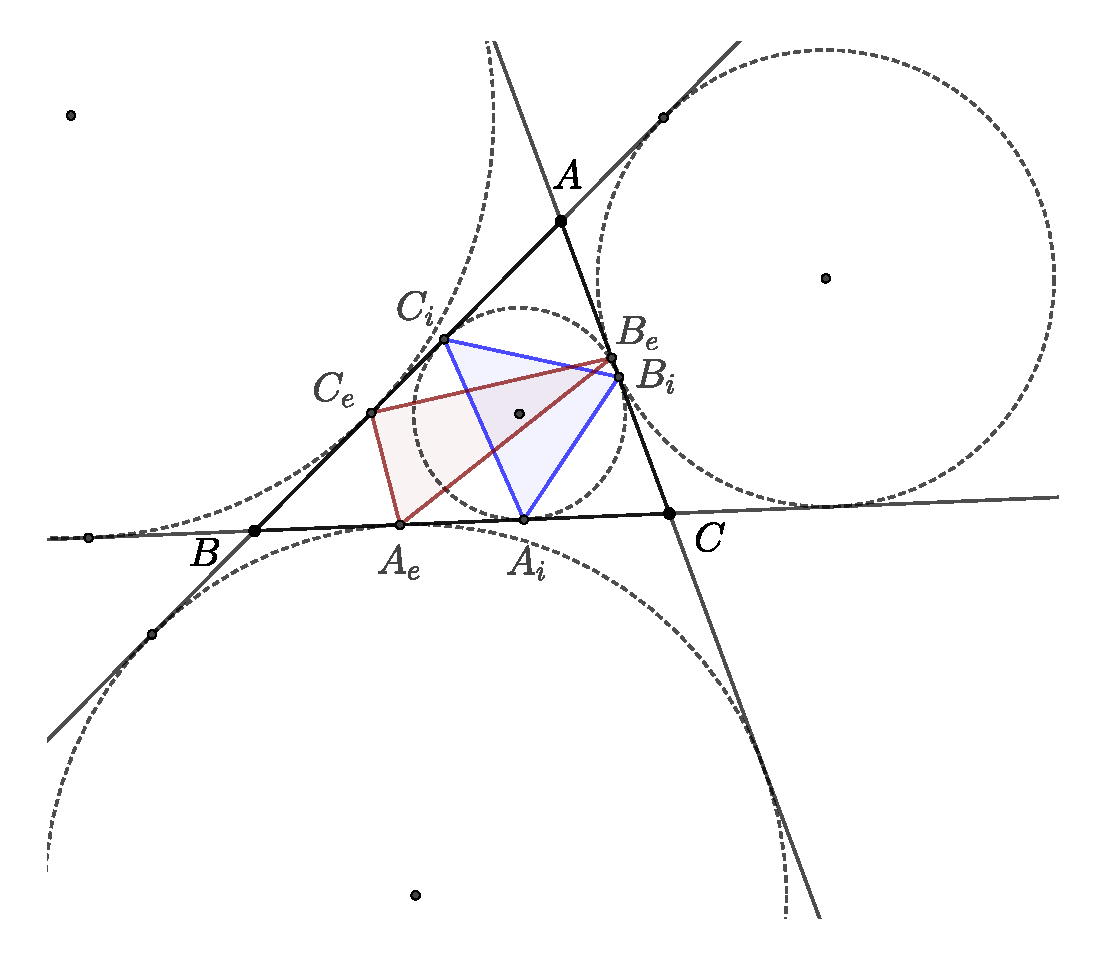
\includegraphics[scale=0.4]{zappA/pics/pics-appA-intouch-extouch.pdf}
    \caption{Intouch triangle (blue) and extouch triangle (brown).}
    \label{fig:appA-intouch-extouch}
\end{figure}

The extouch points are midpoints of the perimeter of $T$. For example, $|A-C|+|A-C_e|=|B-C|+|B-C_e|$. Also, the extouch points are in the caustic (Mandart innelipse) of an elliptic billiard having $T=ABC$ as 3-periodic orbit.

The trilinear vertex matrix of the intouch triangle is given by:
\begin{align*}
    \left(\begin{matrix}
    0 &\frac{ac}{a-b+c} &\frac{ab}{a+b-c}\\
     \frac{bc}{-a+b+c} & 0 &\frac{ab}{a+b-c}\\
       \frac{bc}{-a+b+c}   &\frac{ac}{a-b+c}&0  
    \end{matrix}\right)
\end{align*}

The trilinear vertex matrix of the extouch triangle is given by:
\begin{align*}
    \left(\begin{matrix}
    0 &\frac {a-b+c}{b} &\frac{a+b-c}{c}\\
     \frac{-a+b+c}{a} & 0 &\frac{a+b-c}{c}\\
       \frac{-a+b+c}{a}   &\frac{a-b+c}{b}&0  
    \end{matrix}\right)
\end{align*}

\subsection{Pedal and Antipedal Triangles}

Given a triangle $T=ABC$  and a point $P$ which is not a vertex of $T$ drop three perpendiculars to the sidelines of $T$. The intersections of theses lines with the sidelines define a triangle $T'=A'B'C'$ that is known as the {\em pedal triangle} of $P$. See \cref{fig:appA-pedal-triangle}, left.

The antipedal triangle is defined by the following construction.
Drop half lines from $P$ to the vertices of the triangle $T$. For each vertex draw a line perpendicular to the correspondent half  line. The intersections of these  lines will be the vertices of the {\em antipedal triangle}. See \cref{fig:pedal-triangle}, right.
 \begin{figure}[H]
    %\centering
  % 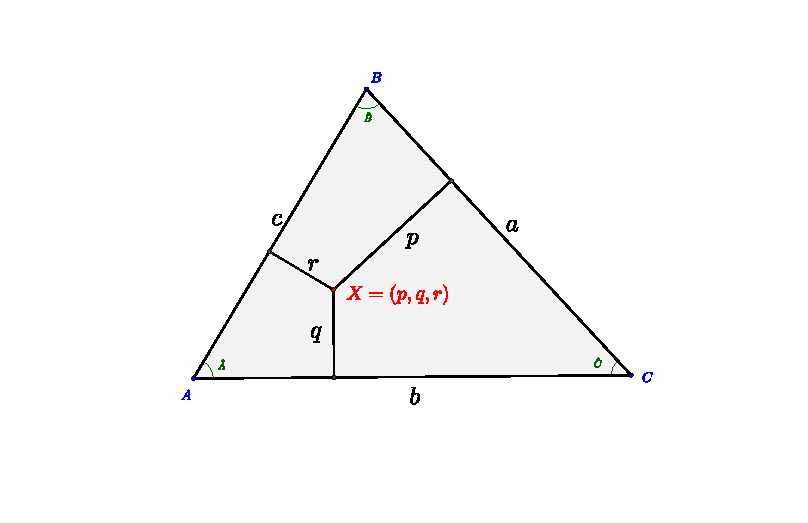
\includegraphics[scale=0.5]{trilinear.pdf}
      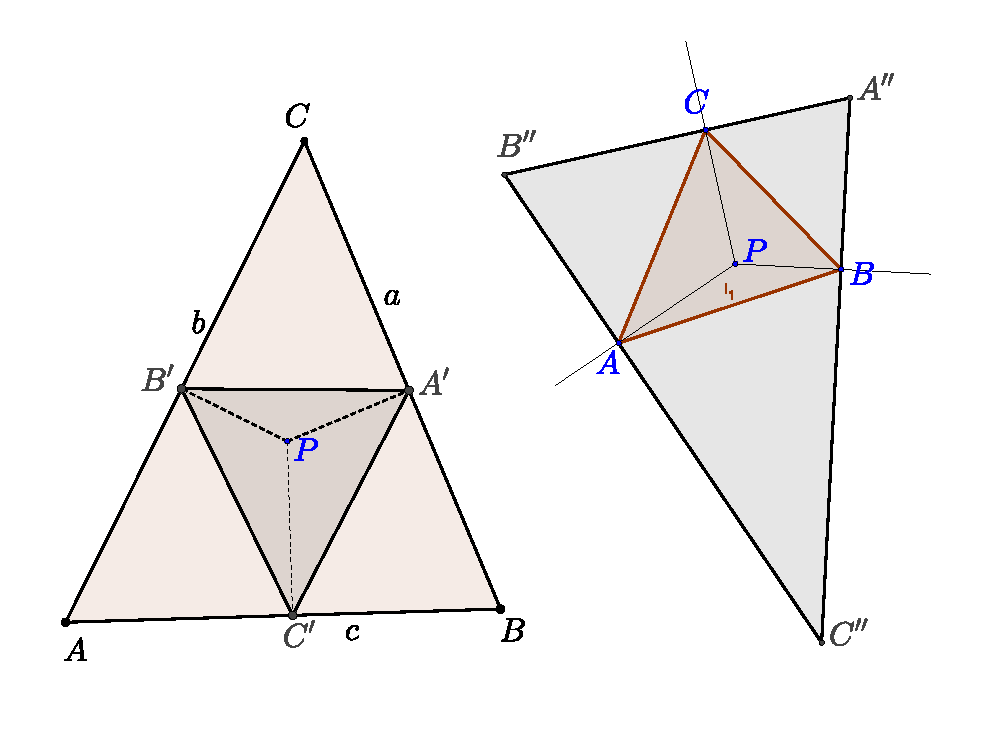
\includegraphics[scale=0.6]{pics_appA_050_pedal_antipedal_triangle.pdf}
    \caption{Pedal triangle $A'B'C'$ of the point $P$.}
    \label{fig:appA-pedal-triangle}
\end{figure}

Let $P=[p,q,r]$ given in trilinear coordinates. The trilinear vertex matrix of the pedal triangle $T'=A'B'C'$ is given by \cite{mw}:

\begin{align*}
   \left(\begin{matrix} 0& q+p\cos C& r+p\cos B\\
   p+q\cos C &0 & r+q\cos A\\
   p+r\cos B & q+r\cos A &0\end{matrix}\right)
\end{align*}


The trilinear vertex matrix of the antipedal triangle $T''=A''B''C''$ is given by \cite{mw}:
 
\begin{align*}
   \left(\begin{matrix} - \frac{ q + p \cos C}{r + p \cos B}& \frac{r + p \cos B}{p + q \cos C}& \frac{q + p \cos C}{p + r \cos B}\\
    \frac{ (r + q \cos A)}{q + p \cos C}& -\frac{r + q \cos A}{p + q \cos  C}& \frac{q + p \cos C}{q + r \cos A}\\
   \frac{q + r \cos A}{r + p \cos B}&\frac{ p + r \cos B}{r + q \cos A} & - \frac{p + r \cos B}{q + r \cos A}\end{matrix}\right)
\end{align*}

 The pedal triangle associated to  $P=X_4$ (orthocenter) is called the {\em orthic triangle}.
 
 For $P=X_1$ (resp. $X_3$) the pedal is the intouch triangle (resp. medial triangle). 
 
 The antipedal of $X_1$ is the excentral triangle.

The notion of pedal triangle  can be generalized for any polygon. From $P$ drop perpendicular half lines to the sidelines (extended) of the polygon. The intersections are the vertices of the {\em pedal polygon.}

Also the {\em  antipedal polygon} is defined analogously to the antipedal triangle.
 
 \subsection{ Anticomplementary triangle}
 
 The anticomplementary triangle of a triangle $T=ABC$ is the triangle $T'=A'BC'$ such that $T$ is the medial triangle of $T$.
 
  \begin{figure}[H]
     \centering
      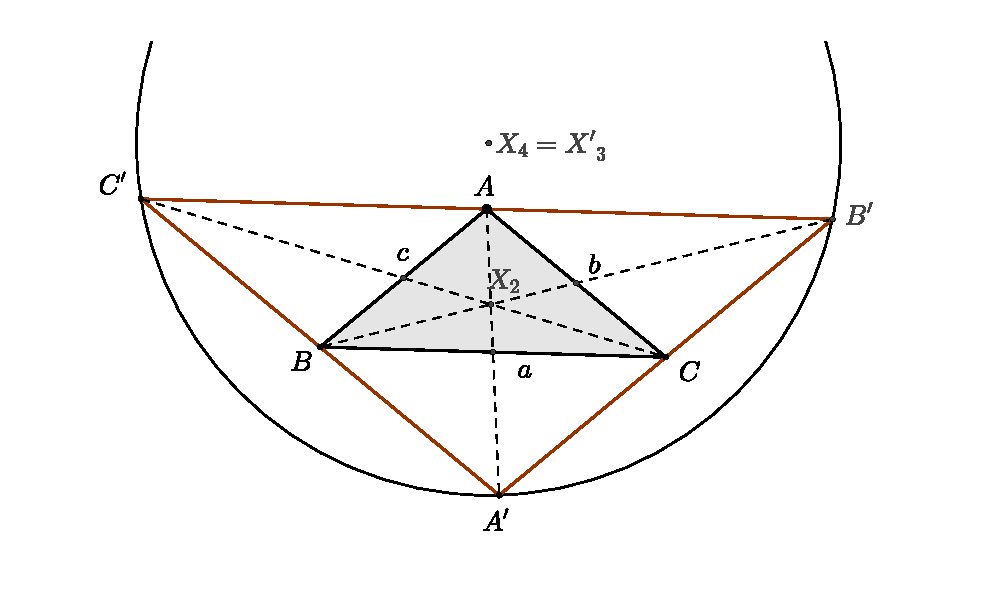
\includegraphics[scale=0.6]{zappA/pics/pics_appA_0100_anticimplementary.pdf}
    \caption{Anticomplementary triangle $A'B'C'$ of $ABC$.}
    \label{fig:pedal-triangle}
\end{figure}
The center of the circumcircle of $T'$ coincides with the orthocenter of $T$, i.e., $X'_3=X_4$.

The trilinear vertex matrix of the antipedal triangle $T'=A'B'C'$ is given by \cite{mw}:
 
\begin{align*}
   \left(\begin{matrix}-\frac{1}{a} &\frac{1}{b} &\frac{1}{c}\\
    \frac{1}{a} &-\frac{1}{b} &\frac{1}{c}\\
    \frac{1}{a} &\frac{1}{b} &-\frac{1}{c}\end{matrix}\right)
    \end{align*}
   
   \section{Ceva Triangle}
   
   Given a triangle $ABC$ and a point $P$, draw the lines $AP$, $BP$, $CP$. The intersections of these lines with the opposite sidelines of $T$ define a triangle $A_1B_1C_1$ which is called {\em Ceva triangle}, see \cref{fig:appA-ceva-triangle}
   
     \begin{figure}[H]
     \centering
      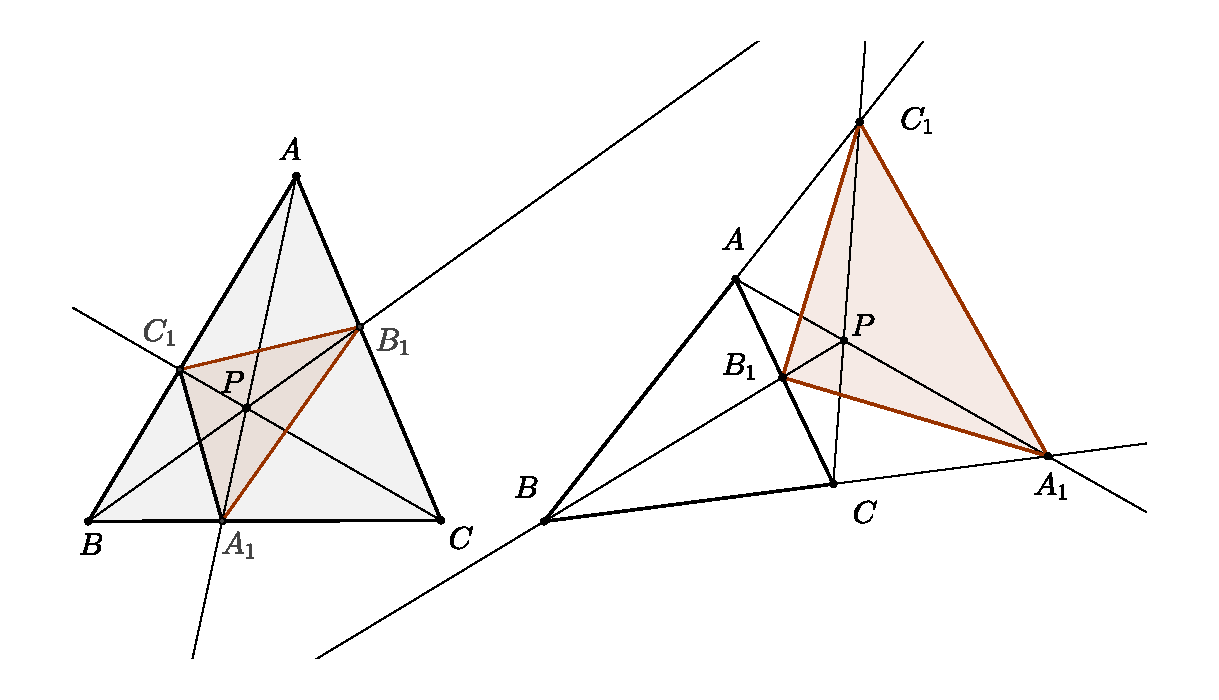
\includegraphics[scale=0.4]{pics-appA-120-ceva.pdf}
    \caption{Ceva triangle $A_1B_1C_1$ of $ABC$.}
    \label{fig:appA-ceva-triangle}
\end{figure}
Let $P=[p,q,r]$. The trilinear vertex matrix of the Ceva triangle $A_1B_1C_1$ is given by:
\[
\left( \begin{matrix}  0 & q & r \\  p & 0 & r
\\p & q & 0 \end{matrix} \right) \]


\section{Feuerbach Triangle}

Given a triangle $ABC$ consider the 9-point circle and the three external circles. The points of contact between the circles define the so called {\em Feuerbach triangle}. See \cref{fig:appA-feurbach-triangle}

   \begin{figure}[H]
     \centering
      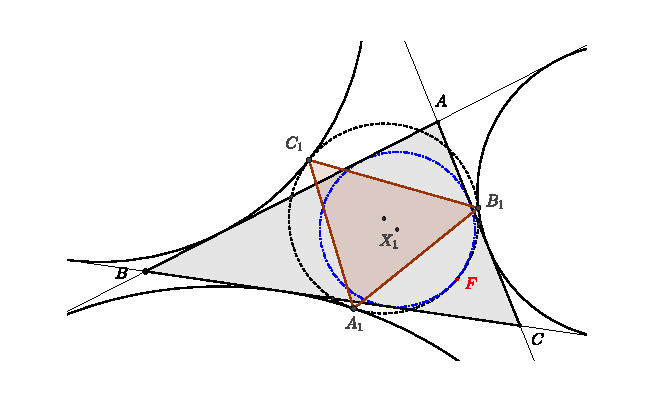
\includegraphics[scale=0.9]{zappA/pics/pics-appA-130-feurbach-triangle.pdf}
    \caption{Feurbach triangle $A_1B_1C_1$ of $ABC$. The point $F=X_{11}$ is the Feurbach point.}
    \label{fig:appA-feurbach-triangle}
\end{figure}


The trilinear vertex matrix of the Feurbach triangle $A_1B_1C_1$ is given by, \cite[Feurbach triangle]{mw}:
\begin{align*}
  \left(\begin{matrix}-\sin^2(\frac{B-C}{2}) & \cos^2(\frac{C-A}{2})  & \cos^2(\frac{A-B}{2})\\ \cos^2(\frac{B-C}{2}) & -\sin^2(\frac{C-A}{2}) & \cos^2(\frac{A-B}{2})\\ \cos^2(\frac{B-C}{2}) & \cos^2(\frac{C-A}{2}) & -\sin^2(\frac{A-B}{2})\end{matrix}\right)
\end{align*}
The trilinear coordinates of $X_{11}$ is given by:
\[[ 1 - \cos(B - C) : 1 - \cos(C - A) : 1 - \cos(A - B)]\]